%%%%%%%%%%%%%%%%%%%%%%%%%%%%%%%%%%%%%%%%%%%%%%%%%%%%%%%%%%%%%%
% https://es.sharelatex.com/learn/Pgfplots_package#/Plotting_mathematical_expressions
%%%%%%%%%%%%%%%%%%%%%%%%%%%%%%%%%%%%%%%%%%%%%%%%%%%%%%%%%%%%%%


\section{Introducción}
%\subsection{Redes neuronales}
El primer modelo de red neuronal artificiales (NN) fue propuesto en 1943 por McCulloc y Pitts en términos de un modelo computacional de actividad nerviosa. Las NN se han inspirado en las redes neuronales biológicas y las conexiones que construyen. Este modelo era un modelo binario, donde cada neurona posee un umbral, y sirvió de base para los modelos posteriores.

Las características principales de las NN son las siguientes:
\begin{enumerate}
	\item Auto-organización y adaptabilidad: utilizan algoritmos de aprendizaje adaptativo y auto-organizativo, por lo que ofrecen mejores posibilidades de procesado robusto y adaptativo.

	\item Procesado no lineal: aumenta la capacidad de la red para aproximar funciones, clasificar patrones y aumenta su inmunidad frente al ruido.

	\item Procesado paralelo: normalmente se usa un gran número de nodos de procesado, con alto nivel de interconectividad.
\end{enumerate}

\subsection{El perceptrón simple}
\begin{imagen}
	\scalebox{1.5}{\begin{tikzpicture}
	%\node [circle split, draw, rotate=90, inner sep=-1pt]  (neurona) at (0, 0) {\rotatebox{-90}{\scriptsize $\sum$} \nodepart{lower} \rotatebox{-90}{\scriptsize $f(z)$}};
	\node [circle, draw, inner sep=1pt] (neurona) at (0, 0) {\scriptsize $\sum_i w_{i}x_{i}$};

	\node (in_0) at (-2.5, 1.5) {$x_0$};
	\node (in_1) at (-2.5, 0.5) {$x_1$};
	\node (in_2) at (-2.5, -0.5) {$x_2$};
	\node (in_n) at (-2.5, -1.5) {$x_n$};
	\node (out) at (2.0, 0.0) {$y_0$};

	\node (d2) at ($(in_2)!0.5!(in_n)$) {$\mathbf{\vdots}$};


	\draw[->] (in_0) -- node[above, pos=0.40] {\scriptsize$w_0$} (neurona);
	\draw[->] (in_1) -- node[above, pos=0.40] {\scriptsize$w_1$} (neurona);
	\draw[->] (in_2) -- node[above, pos=0.40] {\scriptsize$w_i$} (neurona);
	\draw[->] (in_n) -- node[above, pos=0.40] {\scriptsize$w_n$} (neurona);
	\draw[->] (neurona) -- node[above] {$f$} (out);
\end{tikzpicture}
}
	\caption{Perceptrón simple}
	\label{fig:perceptron}
\end{imagen}

\subsection{Las redes neuronales}
El elemento básico de las NN es el nodo, que recibe un vector de entrada para producir una salida como muestra en la figura \ref{fig:perceptron}. Cada entrada tiene asociado un vector de pesos $w$, que se va modificando durante el proceso de aprendizaje. Cada unidad aplica una función $f$ sobre la suma de las entradas ponderada por el vector de pesos como en la ecuacion \ref{eq:entrada}.
\begin{eqnarray}
	y_{i} = \sum_{j} w_{ij}y_{j}\label{eq:entrada}
\end{eqnarray}
Donde el resultado puede servir como entrada de otras unidades.

Existen dos fases importante dentro del modelo
\begin{itemize}
	\item Fase de entrenamiento: Se usa un conjunto de datos o patrones de entrenamiento para determinar los pesos que definen el modelo de la NN. Se calculan de manera iterativa, de acuerdo con los valores de entrenamiento, con el objeto de minimizar el error cometido entre la salida obtenida por la NN y la salida deseada.

	\item Fase de prueba: Durante el entrenamiento, el modelo se ajusta al conjunto de entrenamiento, perdiendo la habilidad de generalizar su aprendizaje a casos nuevos, a esta situación se le llama sobreajuste.
	Para evitar el sobreajuste, se utiliza un segundo grupo de datos diferentes, el conjunto de validación, que permitirá controlar el proceso de aprendizaje.
\end{itemize}
Los pesos óptimos se obtienen minimizando una función. Uno de los criterios utilizados es la minimización del error cuadrático medio entre el valor de salida y el valor real esperado.









\subsection{El perceptrón multicapa}
El perceptrón multicapa es una generalización del perceptrón simple, y surgió como consecuencia de las limitaciones de dicha arquitectura para resolver problemas de clasificación no lineal. Minsky y Papert \cite{Newell1969b} mostraron que el uso de varios perceptrones simples podía resultar una solución para resolver problemas no lineales. Sin embargo, dicha propuesta no presentaba una solución al problema de la actualización de los pesos de las capas, pues la regla de aprendizaje del perceptrón simple no era aplicable. Rummelhart, Hinton y Wilians presentaron la {\em regla delta generalizada}, una forma de propagar el error de la red desde la capa de salida hacia las capas anteriores.

Las redes neuronales, el perceptrón multicapa es una de las arquitecturas más usadas para resolver problemas. Esto es debido a que poseen la capacidad de ser un aproximador universal. Esto no implica que sea una de las redes más potentes o con mejores resultados, el perceptrón multicapa posee una serie de limitaciones, como el proceso de aprendizaje para problemas que dependan de un gran número de variables, la dificultad para realizar un análisis teórico de la red debido a la presencia de componentes no lineales y a la alta conectividad.

\subsubsection{Arquitectura}
El perceptron multicapa posee una estructura de capas compuestas por neuronas. Cada una de las capas está formada por un conjunto de neuronas y se distinguen tres tipos de capas: la capa de entrada, las capas ocultas y la capa de salida.

Las neurones de la capa de entrada se encargan de recibir los patrónes y propagar dichas señales a las neuronas de la capa siguiente. La última capa, la capa de salida, proporciona la respuesta de la red al patrón presentado. Las neuronas de las capas ocultas realizan el procesado de las señales generadas por el patrón de entrada.
\begin{imagen}
	\scalebox{0.8}{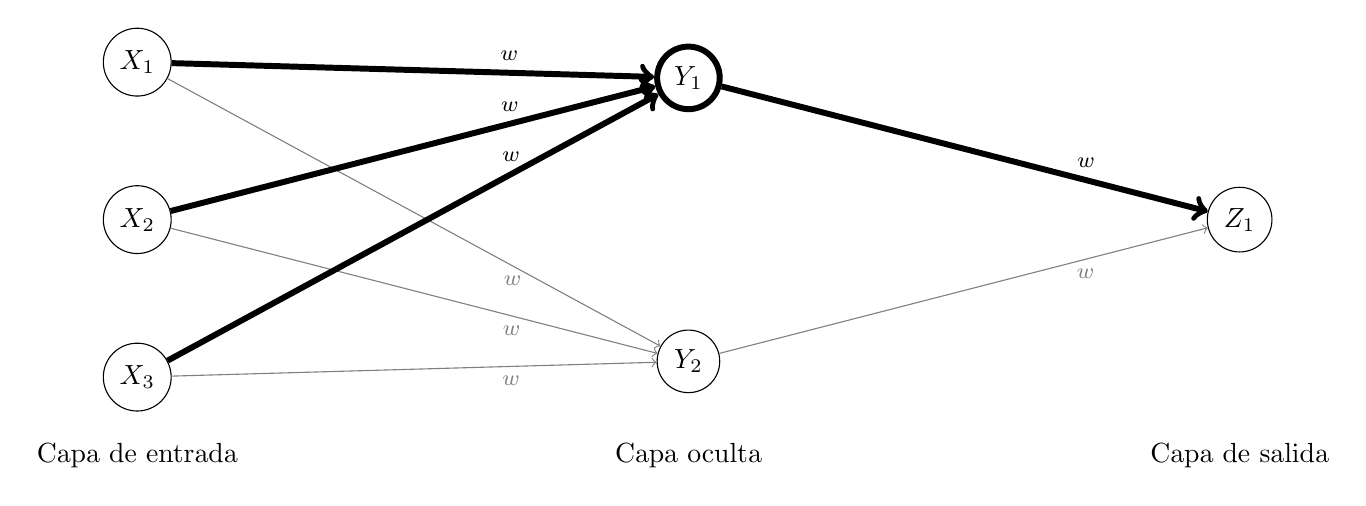
\begin{tikzpicture}

	\tikzstyle{nodo}=[circle, draw, minimum size=5ex]
	\tikzstyle{upw}=[dashed, red, ->, line width = 1pt]
	\tikzstyle{bold}=[line width=0.5ex]

	\coordinate (l_0) at (0, 3.5);
	\coordinate (l_1) at (7, 3.5);
	\coordinate (l_2) at (14, 3.5);
	\coordinate (input) at (0, -3.0);
	\coordinate (hidden) at (7, -3.0);
	\coordinate (output) at (14, -3.0);

	\coordinate (f_1_1) at (0, 2.0); % CAPA ENTRADA
	\coordinate (f_1_2) at (0, 0); % CAPA ENTRADA
	\coordinate (f_1_3) at (0, -2.0); % CAPA ENTRADA
	\coordinate (f_2_1) at (7, 1.8); % CAPA OCULTA 1
	\coordinate (f_2_2) at (7, -1.8); % CAPA OCULTA 1
	\coordinate (f_3_1) at (14, 0); % CAPA SALIDA

	%\node[] (l_0) at (l_0) {$L - 1$};
	%\node[] (l_1) at (l_1) {$L$};
	%\node[] (l_2) at (l_2) {$L + 1$};
	\node[] (input) at (input) {Capa de entrada};
	\node[] (hidden) at (hidden) {Capa oculta};
	\node[] (output) at (output) {Capa de salida};

	\node[nodo] (f_1_1) at (f_1_1) { $X_1$}; % CAPA ENTRADA
	\node[nodo] (f_1_2) at (f_1_2) { $X_2$}; % CAPA ENTRADA
	%\node[nodo] (f_1_3) at (f_1_3) {\Large $f_i(e_i)$}; % CAPA ENTRADA
	\node[nodo] (f_1_3) at (f_1_3) { $X_3$}; % CAPA ENTRADA
	\node[nodo, bold] (f_2_1) at (f_2_1) { $Y_1$}; % CAPA OCULTA 1
	\node[nodo] (f_2_2) at (f_2_2) { $Y_2$}; % CAPA OCULTA 1
	\node[nodo] (f_3_1) at (f_3_1) { $Z_1$}; % CAPA SALIDA


	\draw[->, font=\footnotesize, gray] (f_1_1) -- node[pos=0.70, below] (w_2_1) {$w$} (f_2_2);
	\draw[->, font=\footnotesize, gray] (f_1_2) -- node[pos=0.70, below] (w_2_2) {$w$} (f_2_2);
	\draw[->, font=\footnotesize, gray] (f_1_3) -- node[pos=0.70, below] (w_2_3) {$w$} (f_2_2);
	\draw[->, font=\footnotesize, bold] (f_1_1) --  node[pos=0.7, above] (w_1_1) {$w$} (f_2_1);
	\draw[->, font=\footnotesize, bold] (f_1_2) --  node[pos=0.70, above] (w_1_2) {$w$} (f_2_1);
	\draw[->, font=\footnotesize, bold] (f_1_3) -- node[pos=0.70, above] (w_1_3) {$w$} (f_2_1);

	\draw[->, font=\footnotesize, gray] (f_2_2) -- node[near end, below] {$w$} (f_3_1);
	\draw[->, font=\footnotesize, bold] (f_2_1) -- node[near end, above ] (w_j_k) {$w$} (f_3_1);
\end{tikzpicture}
}
	\caption{Neurona}
	\label{fig:neurona}
\end{imagen}

En la figura \ref{fig:neurona} se observa que las conexiones van siempre hacia adelante, es decir, las neuronas de la capa $l$ se conectan con las neuronas de la capa $l + 1$. Las neuronas de una capa están conectadas a todas las neuronas de la capa siguiente.

\subsubsection{Propagación de la entrada}
El perceptrón multicapa define una relación entre la entrada y la salida. Esta relación se obtiene propagando hacia adelante los valores de las variables de entrada, es por esto que también se les llama redes {\em feedforward}. Cada neurona de la red procesa la entrada recibida y produce una respuesta que se propaga, mediante las conexiones, hacia las neuronas de la capa siguiente.

Si un perceptrón multicapa con $C$ capas y $n_c$ neuronas en la capa $c$, donde $W_c = (w^{c}_{ij})$ es la matriz de pesos, donde $w^{c}_{ij}$ representa el peso de la conexion de la neurona $i$ de la capa $c$. Denotaremos $a^{c}_{i}$ a la activación de la neurona $i$ de la capa $c$ que se calcula de la siguiente manera
\begin{itemize}
	\item Activación de una neurona de la capa de entrada: Las neuronas se encargan de transmitir la entrada recibida, por lo tanto $$ a^{1}_{i} = x_{i}, i = 1, 2, \cdots, n$$ donde $X = (x_1, x_2, \cdots, x_n)$ representa el vector de entrada.

	\item Activación de una neurona de la capa oculta: Las neuronas de una capa oculta procesa la información recibida aplicando la función de activación $f$ a la suma de los productos de la entrada por sus pesos, es decir $$ a^{c}_{i} = f\left(\sum^{n_{c - 1}}_{j=1} w^{c - 1}_{ji}a^{c - 1}_{j} + \theta^{c}_{i}\right), i = 1, 2, \cdots, n_c; c = 2, 3, \cdots, C - 1$$ donde $a^{c - 1}_{j}$ es la salida de la capa anterior a $c$.

	\item Activación de una neurona de la capa de salida: La activación de una neurona de la capa de salida viene dada por la función de activación $f$ aplicada a la suma de los productos de la entrada por sus pesos, es decir $$ y_{i} = a^{c}_{i} = f\left(\sum^{n_{c - 1}}_{j=1} w^{C - 1}_{ji}a^{C - 1}_{j} + \theta^{C}_{i}\right), i = 1, \cdots, n_c$$ donde $Y = (y_1, y_2, \cdots, y_{n_{c}})$ es el vector de salida.
\end{itemize}

La función $f$ es la función de activación de la neurona. Las funciones de activación mas utilizadas son la sigmoidal y la tangente hiperbólica (ver ecuación \ref{eq:sigm} y \ref{eq:tanh} respectivamente).
\begin{eqnarray}
	f_{sigm}(x) &=& \frac{1}{1+\exp(-x)}\label{eq:sigm}
\end{eqnarray}
\begin{eqnarray}
	f_{tanh}(x) &=& \frac{1 - \exp(-x)}{1 + \exp(-x)}\label{eq:tanh}
\end{eqnarray}

Ambas funciones poseen como imagen intervalo de valores entre $[0, 1]$ y $[-1, 1]$ como se observa en la figura \ref{fig:funciones}.% y están descritas por las ecuaciones \ref{eq:sigm} y \ref{eq:tanh}.

\begin{imagen}
	\scalebox{1.0}{
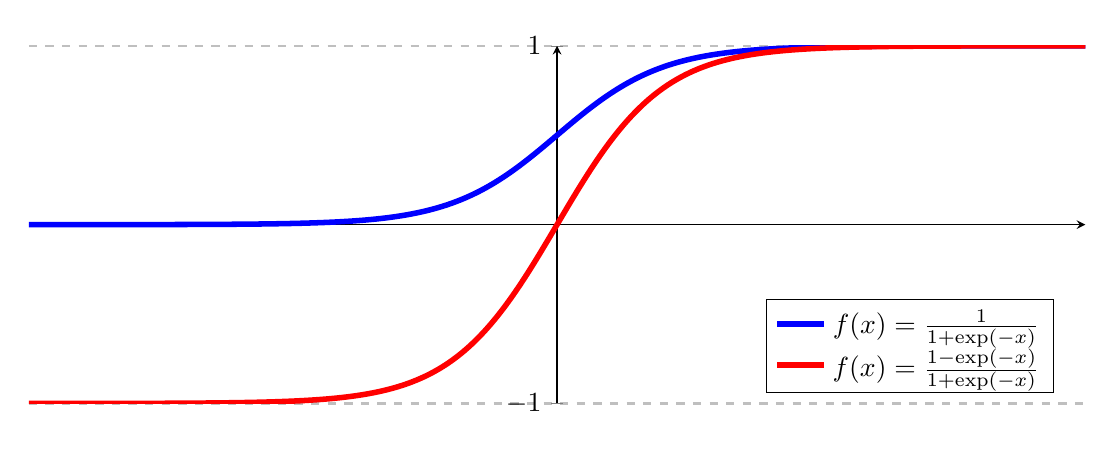
\begin{tikzpicture}
\begin{axis}[ymin=-1, ymax = 1, axis lines = left, legend pos=south east, width=15cm, xmajorticks=false, ytick={-1, +1}, axis lines=middle, y post scale=0.4, ymajorgrids=true, major grid style={dashed, line width=0.8pt}, yticklabel pos=left]
%Here the blue parabloa is defined
\addplot[domain=-10:10, samples=1000, color=blue, line width=2pt]{1/(1 + exp(-x))};
\addplot[domain=-10:10, samples=1000, color=red, line width=2pt]{(1 - e^(-x))/(1 + e^(-x))};
\addlegendentry{$f(x) = \frac{1}{1+\exp(-x)}$}
\addlegendentry{$f(x) = \frac{1 - \exp(-x)}{1 + \exp(-x)}$}
\end{axis}
%\begin{axis}[ymin=-1, ymax = 1, axis lines = left, xlabel = $x$, ylabel = {$f(x)$}]
%%Here the blue parabloa is defined
%\addplot[domain=-10:10, samples=1000, color=red]{(1 - e^(-x))/(1 + e^(-x))};
%\addlegendentry{$(1 - \exp(-x))/(1 + \exp(-x))$}
%\end{axis}
\end{tikzpicture}
% 1/(1+exp(-x))
}
	\caption{Funciones de activación mas utilizadas.}
	\label{fig:funciones}
\end{imagen}



%\begin{imagen}
%	\scalebox{1.0}{\input{img/tangente}}
%	\caption{Función tangente}
%\end{imagen}
